\documentclass[a4paper,12pt]{article}

\usepackage[english]{babel}
\usepackage[T1]{fontenc}
\usepackage[utf8]{inputenc}
\usepackage{lmodern}
\usepackage{geometry}
\geometry{margin=2.5cm}
\usepackage{graphicx}
\usepackage{float}
\usepackage{array}
\usepackage{tabularx}
\usepackage{booktabs}
\usepackage{listings}
\usepackage{xcolor}
\usepackage{hyperref}

\definecolor{codegray}{rgb}{0.96,0.96,0.96}
\definecolor{commentgreen}{rgb}{0,0.5,0}
\definecolor{keywordblue}{rgb}{0,0,0.7}

\lstset{
    backgroundcolor=\color{codegray},
    basicstyle=\ttfamily\small,
    breaklines=true,
    commentstyle=\color{commentgreen},
    keywordstyle=\color{keywordblue},
    frame=single,
    language=bash,
    showstringspaces=false,
    captionpos=b,
    numbers=left,
    numberstyle=\tiny\color{gray}
}

\hypersetup{
    colorlinks=true,
    linkcolor=black,
    urlcolor=blue,
    pdftitle={TP1 Report - RabbitMQ},
    pdfauthor={Aymen Abid, Mohamed Yassine Kallel}
}

\newcommand{\HRule}[1]{\rule{\linewidth}{#1}}
\newcommand{\InsertLogo}[1]{%
    \IfFileExists{#1}{\includegraphics[width=2.5cm]{#1}}{\fbox{\parbox[c][2.5cm][c]{2.5cm}{\centering Logo}}}%
}

\title{TP1 Report - Introduction to RabbitMQ for Distributed Applications}
\author{Aymen Abid \and Mohamed Yassine Kallel}
\date{Academic Year 2025--2026}

\begin{document}

\begin{titlepage}
    \centering

    \begin{minipage}{0.2\textwidth}
        \begin{flushleft}
            \InsertLogo{insat.png}
        \end{flushleft}
    \end{minipage}
    \begin{minipage}{0.55\textwidth}
        \centering
        {\small \textbf{REPUBLIC OF TUNISIA}} \\
        {\small Ministry of Higher Education \\ and Scientific Research} \\
        \vspace{0.2cm}
        {\small \textbf{University of Carthage \\ INSAT - National Institute of Applied Science and Technology}}
    \end{minipage}
    \begin{minipage}{0.2\textwidth}
        \begin{flushright}
            \InsertLogo{ucar.png}
        \end{flushright}
    \end{minipage}

    \vspace{0.5cm}
    \HRule{1.5pt} \\ [0.4cm]
    \vspace{2cm}
    {\Huge \textbf{Lab Report}} \\ [0.5cm]
    {\huge \textbf{TP1 - RabbitMQ}} \\ [0.8cm]
    \vspace{7.6cm}

    \begin{minipage}{0.45\textwidth}
        \begin{flushleft}\large
            \textbf{Prepared by:}\\
            Aymen \textsc{Abid} \\
            Mohamed Yassine \textsc{Kallel}
        \end{flushleft}
    \end{minipage}
    \hfill
    \begin{minipage}{0.45\textwidth}
        \begin{flushright}\large
            \textbf{Instructor:}\\
            Mr. Sofiane Ouni
        \end{flushright}
    \end{minipage}

    \vfill
    {\large Academic Year 2025--2026}
\end{titlepage}

\tableofcontents
\newpage

\section*{Abstract}
\addcontentsline{toc}{section}{Abstract}

This report presents the implementation of TP1 on RabbitMQ, keeping the same learning objectives as the original lab sheet while using a Docker-based setup instead of local Erlang and RabbitMQ installation. The work covers broker setup, management interface usage, queue and exchange operations, Java producer and consumer development, and direct-exchange routing for selective log processing. The final result is a reproducible environment where each question of the TP is mapped to code and observable behavior.

\section{Introduction}

Message-oriented middleware decouples distributed application components by replacing direct process-to-process communication with asynchronous exchanges through a broker. RabbitMQ is a widely used AMQP broker that supports queues, exchanges, bindings, acknowledgements, and routing policies.

The objective of this TP is to understand these mechanisms through progressive experiments:

\begin{enumerate}
    \item Start and access a RabbitMQ server.
    \item Manipulate entities from the web interface.
    \item Implement a producer.
    \item Implement a consumer with callback and acknowledgement.
    \item Use a direct exchange with routing keys.
\end{enumerate}

\section{Core Concepts}

\begin{table}[H]
\centering
\begin{tabularx}{\textwidth}{>{\bfseries}l X}
\toprule
Concept & Practical definition used in this TP \\
\midrule
Broker & RabbitMQ server that receives, stores, and routes messages \\
Queue & Buffer where messages wait to be consumed \\
Exchange & Routing component that forwards messages to queues \\
Binding & Rule linking a queue to an exchange, optionally with a key \\
Routing key & String used by exchanges, for example direct exchange, to select queues \\
Producer & Application that publishes messages \\
Consumer & Application that receives messages \\
Acknowledgement & Confirmation from consumer that processing is complete \\
\bottomrule
\end{tabularx}
\caption{Core messaging concepts used in TP1}
\end{table}

\section{Environment and Setup Strategy}

\subsection{Requirement in the original TP}

The lab sheet requests local installation of Erlang and RabbitMQ on Windows, then enabling the management plugin.

\subsection{Equivalent setup used in this work}

To preserve the same educational goals with better reproducibility, this implementation uses Docker Compose:

\begin{itemize}
    \item Compose file: \texttt{compose.yml}
    \item RabbitMQ image: \texttt{rabbitmq:3.13-management}
    \item AMQP port: \texttt{5672}
    \item Management UI port: \texttt{15672}
    \item Default credentials: \texttt{student/student}
\end{itemize}

Startup command:

\begin{lstlisting}
docker compose -f compose.yml up -d
\end{lstlisting}

\section{Project Structure}

\begin{table}[H]
\centering
\begin{tabularx}{\textwidth}{>{\ttfamily}p{0.52\textwidth} X}
\toprule
File & Role \\
\midrule
pom.xml & Java dependencies and execution plugin \\
src/main/java/tp1/RabbitMqConfig.java & ConnectionFactory configuration (host, port, user, password) \\
src/main/java/tp1/Send.java & Producer for queue hello \\
src/main/java/tp1/Receive.java & Consumer with DeliverCallback and explicit acknowledgement \\
src/main/java/tp1/EmitLogDirect.java & Producer to direct exchange direct\_logs \\
src/main/java/tp1/ReceiveLogsDirect.java & Routing-key based consumer for direct exchange \\
\bottomrule
\end{tabularx}
\caption{Files implemented for TP1}
\end{table}

\section{Question-by-Question Mapping}

\subsection{Q1 - Installation}

\textbf{Original request:}
\begin{itemize}
    \item Install Erlang.
    \item Install RabbitMQ server.
\end{itemize}

\textbf{Implemented equivalent:}
\begin{itemize}
    \item Start broker with Docker Compose using \texttt{compose.yml}.
    \item No local Erlang or RabbitMQ executable is required.
\end{itemize}

\textbf{Validation:}
\begin{itemize}
    \item Container status is healthy.
    \item Broker listens on ports \texttt{5672} and \texttt{15672}.
\end{itemize}

\subsection{Q2 - Enable and use web management interface}

\textbf{Original request:}
Enable \texttt{rabbitmq\_management} plugin manually.

\textbf{Implemented equivalent:}
\begin{itemize}
    \item The management plugin is already enabled in \texttt{rabbitmq:3.13-management}.
    \item UI endpoint is \url{http://localhost:15672}.
\end{itemize}

\textbf{Validation:}
\begin{itemize}
    \item Successful login with \texttt{student/student}.
    \item Overview, Exchanges, and Queues tabs are accessible.
\end{itemize}

\subsection{Q3 - Manual queue, exchange, and binding operations in UI}

\textbf{Actions performed in UI:}
\begin{enumerate}
    \item Create exchange.
    \item Create queue.
    \item Bind queue to exchange.
    \item Publish a test message.
    \item Read the message from the queue.
\end{enumerate}

\textbf{Captured evidence:}

\begin{figure}[H]
    \centering
    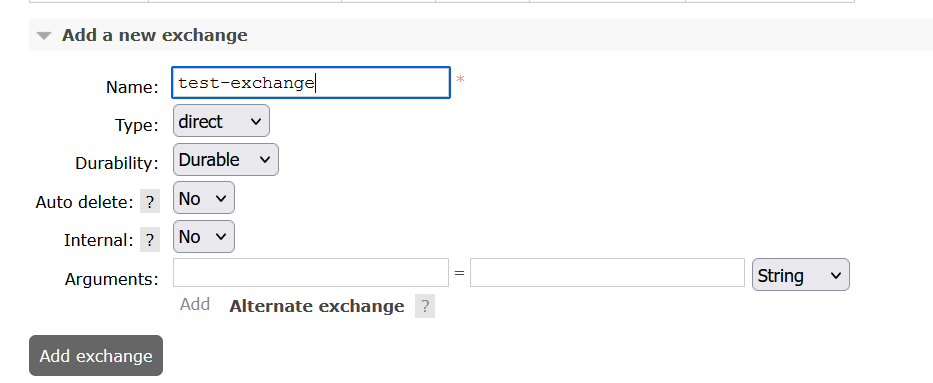
\includegraphics[width=0.92\textwidth]{assets/image.png}
    \caption{Q3 - Adding an exchange}
\end{figure}

\begin{figure}[H]
    \centering
    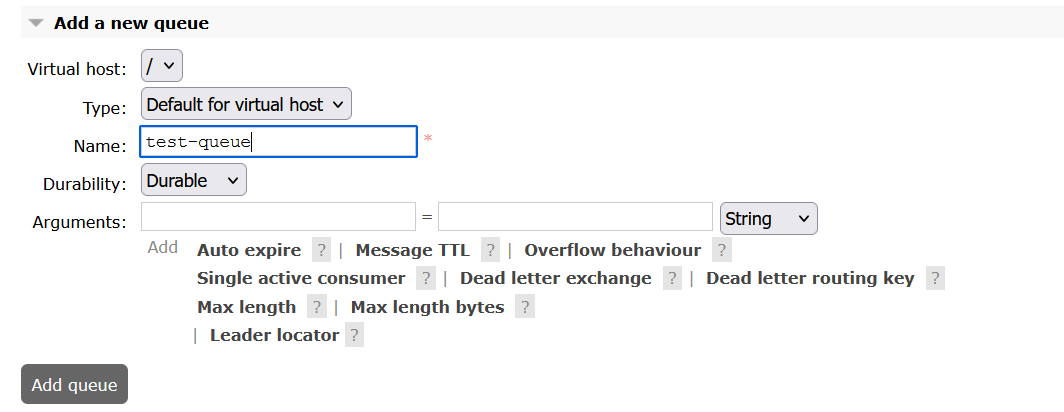
\includegraphics[width=0.92\textwidth]{assets/image-1.png}
    \caption{Q3 - Adding a queue}
\end{figure}

\begin{figure}[H]
    \centering
    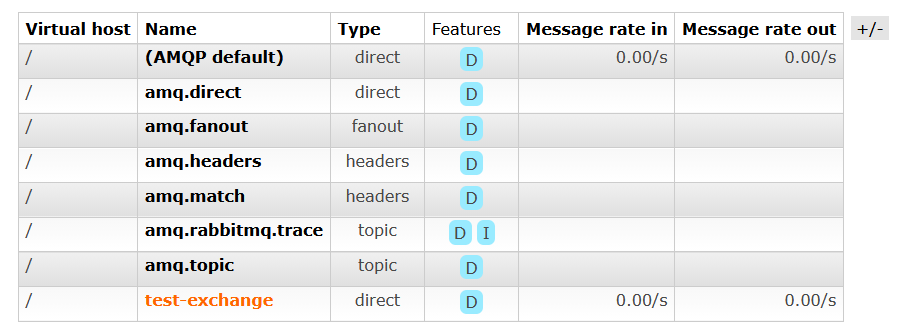
\includegraphics[width=0.92\textwidth]{assets/image-2.png}
    \caption{Q3 - Selecting the exchange}
\end{figure}

\begin{figure}[H]
    \centering
    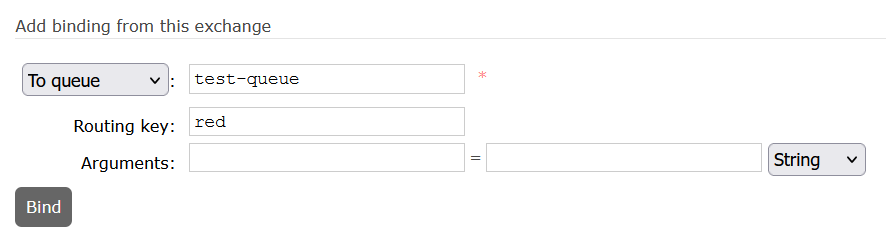
\includegraphics[width=0.92\textwidth]{assets/image-3.png}
    \caption{Q3 - Creating a binding}
\end{figure}

\begin{figure}[H]
    \centering
    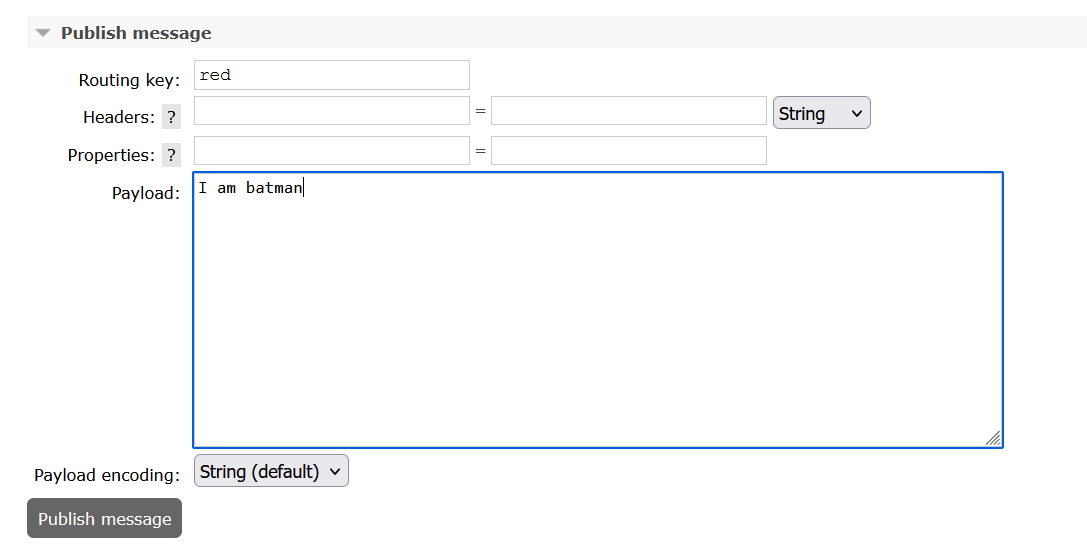
\includegraphics[width=0.92\textwidth]{assets/image-4.png}
    \caption{Q3 - Publishing a message}
\end{figure}

\begin{figure}[H]
    \centering
    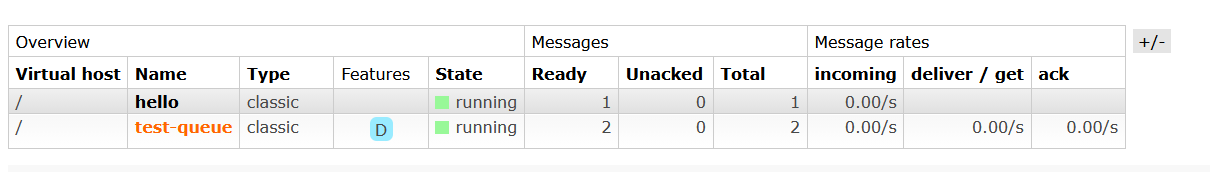
\includegraphics[width=0.92\textwidth]{assets/image-5.png}
    \caption{Q3 - Selecting the queue}
\end{figure}

\begin{figure}[H]
    \centering
    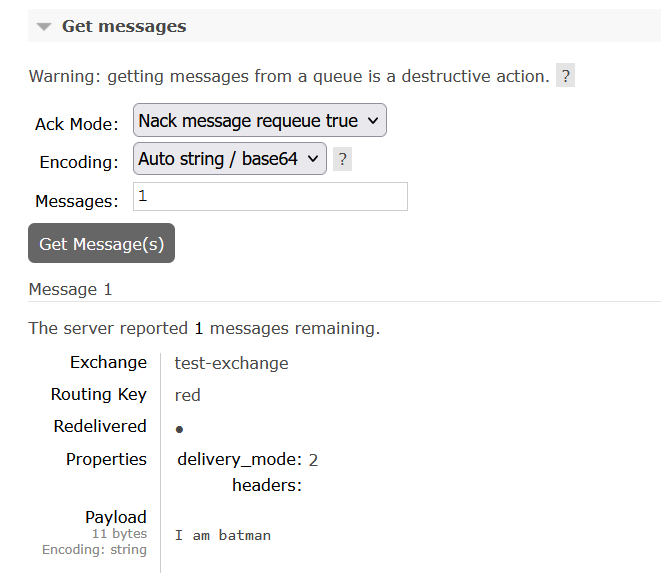
\includegraphics[width=0.92\textwidth]{assets/image-6.png}
    \caption{Q3 - Getting the message}
\end{figure}

\subsection{Q4 - Send client code (hello message)}

\textbf{Implemented in:}
\begin{itemize}
    \item \texttt{src/main/java/tp1/Send.java}
    \item \texttt{src/main/java/tp1/RabbitMqConfig.java}
\end{itemize}

\textbf{Command executed:}

\begin{lstlisting}
mvn -q exec:java '-Dexec.mainClass=tp1.Send' '-Dexec.args=Hello World!'
\end{lstlisting}

\textbf{Expected behavior:}
\begin{itemize}
    \item Queue \texttt{hello} is declared.
    \item Message is published via default exchange to routing key \texttt{hello}.
    \item Terminal prints sent confirmation.
    \item RabbitMQ UI shows queue activity.
\end{itemize}

\textbf{Observed evidence:}

\begin{figure}[H]
    \centering
    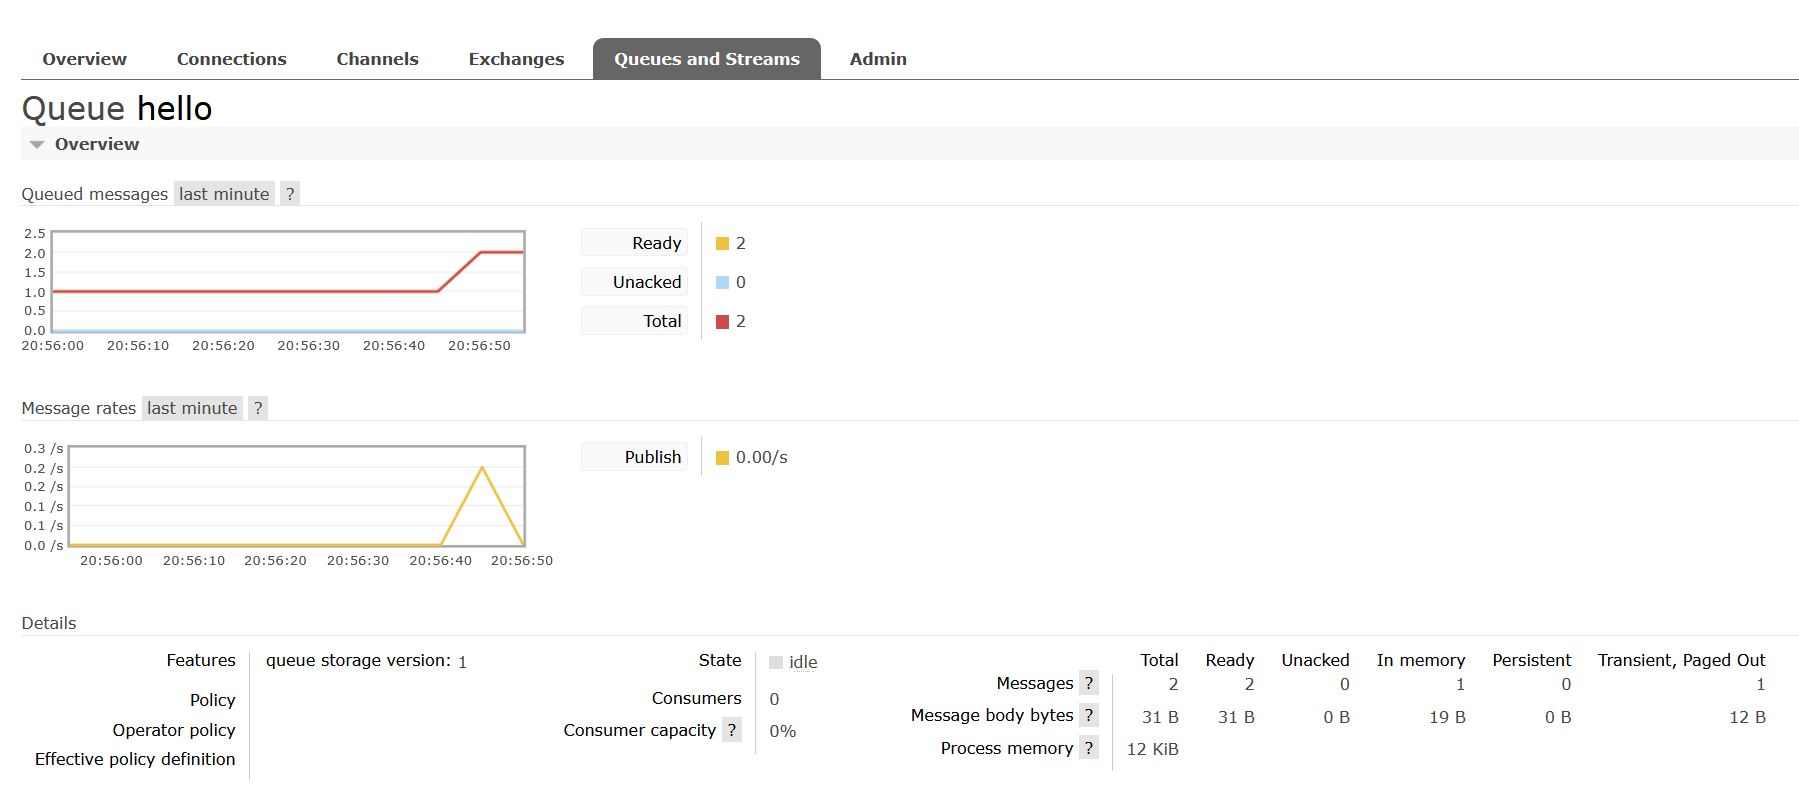
\includegraphics[width=0.92\textwidth]{assets/image-7.png}
    \caption{Q4 - Overview activity after publish}
\end{figure}

\begin{figure}[H]
    \centering
    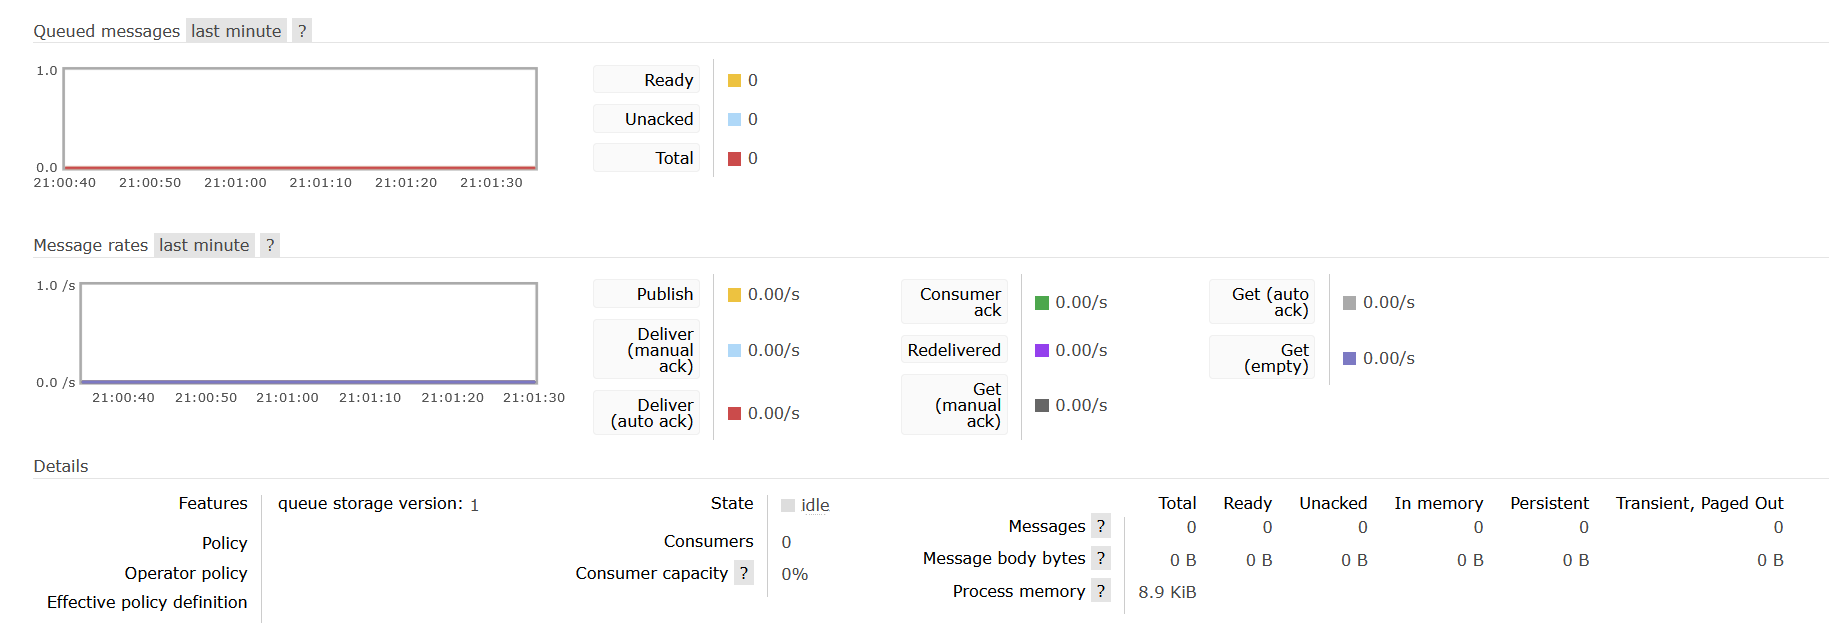
\includegraphics[width=0.92\textwidth]{assets/image-8.png}
    \caption{Q4 - Overview after the activity spike}
\end{figure}

Terminal output:

\begin{lstlisting}
[x] Sent 'Hello World!'
\end{lstlisting}

\subsection{Q5 - Receive client code (consume from queue)}

\textbf{Implemented in:}
\begin{itemize}
    \item \texttt{src/main/java/tp1/Receive.java}
\end{itemize}

\textbf{How this maps to the TP requirement:}
\begin{itemize}
    \item Uses \texttt{DeliverCallback} for asynchronous delivery processing.
    \item Starts a non-exclusive consumer using \texttt{basicConsume}.
    \item Uses explicit acknowledgement with \texttt{autoAck = false} and \texttt{basicAck}.
\end{itemize}

\textbf{Command executed:}

\begin{lstlisting}
mvn -q exec:java '-Dexec.mainClass=tp1.Receive'
\end{lstlisting}

\textbf{Observed terminal excerpt:}

\begin{lstlisting}
[*] Waiting for messages. Press CTRL+C to exit
[x] Received 'healthcheck message'
[x] Received 'Hello World!'
\end{lstlisting}

\subsection{Q6 - Exchange and routing with direct exchange}

\textbf{Implemented in:}
\begin{itemize}
    \item \texttt{src/main/java/tp1/EmitLogDirect.java}
    \item \texttt{src/main/java/tp1/ReceiveLogsDirect.java}
\end{itemize}

\textbf{Experiment setup:}
\begin{enumerate}
    \item Terminal A listens to all severities: info, warning, error.
    \item Terminal B listens only to error and writes output to a file.
    \item Terminal C publishes info, warning, and error messages.
\end{enumerate}

\textbf{Commands used:}

Terminal A:
\begin{lstlisting}
mvn -q exec:java '-Dexec.mainClass=tp1.ReceiveLogsDirect'
\end{lstlisting}

Terminal B:
\begin{lstlisting}
mvn -q exec:java '-Dexec.mainClass=tp1.ReceiveLogsDirect' '-Dexec.args=error' | tee error.log
\end{lstlisting}

Terminal C:
\begin{lstlisting}
mvn -q exec:java '-Dexec.mainClass=tp1.EmitLogDirect' '-Dexec.args=info App started'
mvn -q exec:java '-Dexec.mainClass=tp1.EmitLogDirect' '-Dexec.args=warning High memory'
mvn -q exec:java '-Dexec.mainClass=tp1.EmitLogDirect' '-Dexec.args=error Disk full'
\end{lstlisting}

\textbf{Observed results:}
\begin{itemize}
    \item Terminal A receives all messages.
    \item Terminal B receives only the error message.
    \item \texttt{error.log} is created with the critical line.
    \item RabbitMQ generates queue names for temporary consumers.
\end{itemize}

\begin{figure}[H]
    \centering
    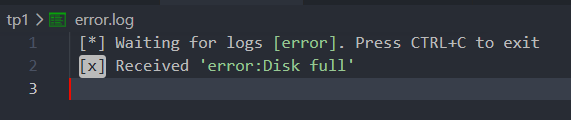
\includegraphics[width=0.92\textwidth]{assets/image-9.png}
    \caption{Q6 - Error log file generated}
\end{figure}

\begin{figure}[H]
    \centering
    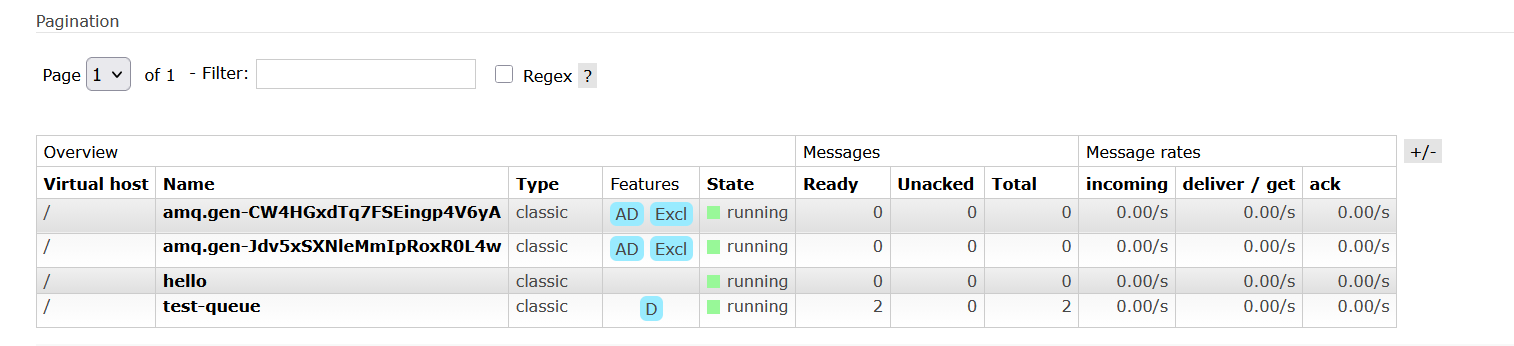
\includegraphics[width=0.92\textwidth]{assets/image-10.png}
    \caption{Q6 - Auto-generated queue name in RabbitMQ UI}
\end{figure}

\section{Results Synthesis}

\begin{table}[H]
\centering
\begin{tabularx}{\textwidth}{>{\bfseries}p{0.55\textwidth} X}
\toprule
TP objective & Result \\
\midrule
Broker installation and accessibility & Achieved with Docker Compose \\
Management interface usage & Achieved and validated with screenshots \\
Producer implementation & Achieved with \texttt{Send.java} \\
Consumer with callback and explicit acknowledgement & Achieved with \texttt{Receive.java} \\
Direct exchange routing & Achieved with \texttt{EmitLogDirect.java} and \texttt{ReceiveLogsDirect.java} \\
\bottomrule
\end{tabularx}
\caption{Summary of objective completion}
\end{table}

\section{Discussion}

\begin{enumerate}
    \item Functional equivalence with the original TP was preserved while replacing local installation with a containerized deployment.
    \item The Docker approach improves reproducibility, cleanup, and onboarding speed.
    \item The Java implementation follows the canonical RabbitMQ tutorial flow while adding explicit acknowledgements in the queue consumer.
    \item Routing experiments clearly demonstrate exact-match behavior of direct exchanges.
\end{enumerate}

\section{Conclusion}

The TP objectives were fully achieved. The final project demonstrates the full RabbitMQ workflow required by the statement: broker setup, web administration, queue operations, producer and consumer coding, and routing with direct exchange. The Docker-based approach keeps the educational content intact while reducing local setup complexity. The project is reproducible and ready for evaluation or extension in future labs.

\section{References}

\begin{enumerate}
    \item TP1 document: MOHAMED YASSINE KALLEL - TP1 RabbitMQ v3.pdf
    \item RabbitMQ official documentation: \url{https://www.rabbitmq.com/docs}
    \item RabbitMQ Java client API: \url{https://rabbitmq.github.io/rabbitmq-java-client/api/current/}
\end{enumerate}

\end{document}